\documentclass[11pt,a4paper]{article}

\usepackage[T1]{fontenc}
\usepackage[utf8]{inputenc}
\usepackage{lmodern}
\usepackage[margin=2.5cm]{geometry}
\usepackage{graphicx}
\usepackage{booktabs}
\usepackage{amsmath,amssymb}
\usepackage{hyperref}
\usepackage{xcolor}
\usepackage{caption}
\usepackage{float}
\usepackage{setspace}

\definecolor{aivancityblue}{HTML}{0B3D5C}
\definecolor{aivancityteal}{HTML}{00D4AA}

\hypersetup{
  colorlinks=true,
  linkcolor=aivancityblue,
  citecolor=aivancityblue,
  urlcolor=aivancityteal
}

% ── Metadata (edit before submission) ──
\newcommand{\reporttitle}{%
  CNN-Adaptive Sliding Mode Control and Reinforcement Learning\\[0.4em]
  for Autonomous Mobile Robot Navigation:\\[0.2em]
  A Digital Twin Approach%
}
\newcommand{\programname}{PGE5 --- AI Clinic Research Report}
\newcommand{\submissiondate}{28 August 2026}
\newcommand{\supervisorname}{Anuradha Kar}

\begin{document}

% ═══════════════════════════════════════
% TITLE PAGE
% ═══════════════════════════════════════
\begin{titlepage}
  \centering
  \vspace*{1cm}

  
\includegraphics[width=0.42\textwidth]{../assets/aivancity_logo.png}\\[1.5cm]

  {\LARGE\bfseries\color{aivancityblue} \reporttitle}\\[1.8cm]

  {\large \programname}\\[2cm]

  \begin{minipage}{0.78\textwidth}
    \centering
    \begin{tabular}{@{}l@{\hspace{1em}}l@{}}
      \textbf{Participating Students} &
      Likhita Yerra \\
      & Mohamed Oussama Bouriga \\
      & Ahmed Ben Aissa \\
      & Abdellahi El Moustapha \\
      & Thibault Goutorbe \\[0.6em]
      \textbf{Supervisor} & \supervisorname \\[0.6em]
      \textbf{Date of Submission} & \submissiondate \\
    \end{tabular}
  \end{minipage}

  \vfill

  {\small aivancity --- School of Technology and Management for AI\\Paris, France}\\[0.3cm]
  {\small \today}
\end{titlepage}

\setcounter{page}{1}
\onehalfspacing

% ═══════════════════════════════════════
% 1. INTRODUCTION
% ═══════════════════════════════════════
\section{Introduction}

\subsection{Problem Statement}

Autonomous mobile robots navigating in unstructured environments must maintain accurate trajectory tracking despite sensor noise, mechanical disturbances, and surface-induced wheel slip. Sliding Mode Control (SMC) is widely adopted in this domain because of its intrinsic robustness to matched disturbances and parameter variations~\cite{utkin1992,edwards1998}. However, classical SMC uses a single fixed set of gains that cannot simultaneously optimise chattering suppression, tracking accuracy, and disturbance rejection across all operating regimes.

When sensors become noisy, fixed gains produce excessive chattering in the angular velocity command. When an external push is applied or wheels lose traction, the same fixed gains may recover too slowly or too aggressively. This motivates \emph{scenario-aware} control: adapting SMC parameters based on the operating environment rather than using one preset for all conditions.

This project addresses the research question:
\begin{quote}
\emph{Can a learning-based perception and control pipeline improve the adaptability of sliding mode control for a differential-drive mobile robot under heterogeneous uncertainty conditions?}
\end{quote}

We propose and evaluate:
\begin{enumerate}
  \item a \textbf{CNN-adaptive SMC} framework that classifies the environment from a 64$\times$64 occupancy map and selects hand-tuned SMC parameter presets;
  \item a \textbf{PPO reinforcement learning agent} that learns continuous SMC gain adaptation from a multi-objective reward signal; and
  \item a \textbf{3D digital twin} web interface for live simulation, controller comparison, replay, and demonstration.
\end{enumerate}

\begin{figure}[H]
  \centering
  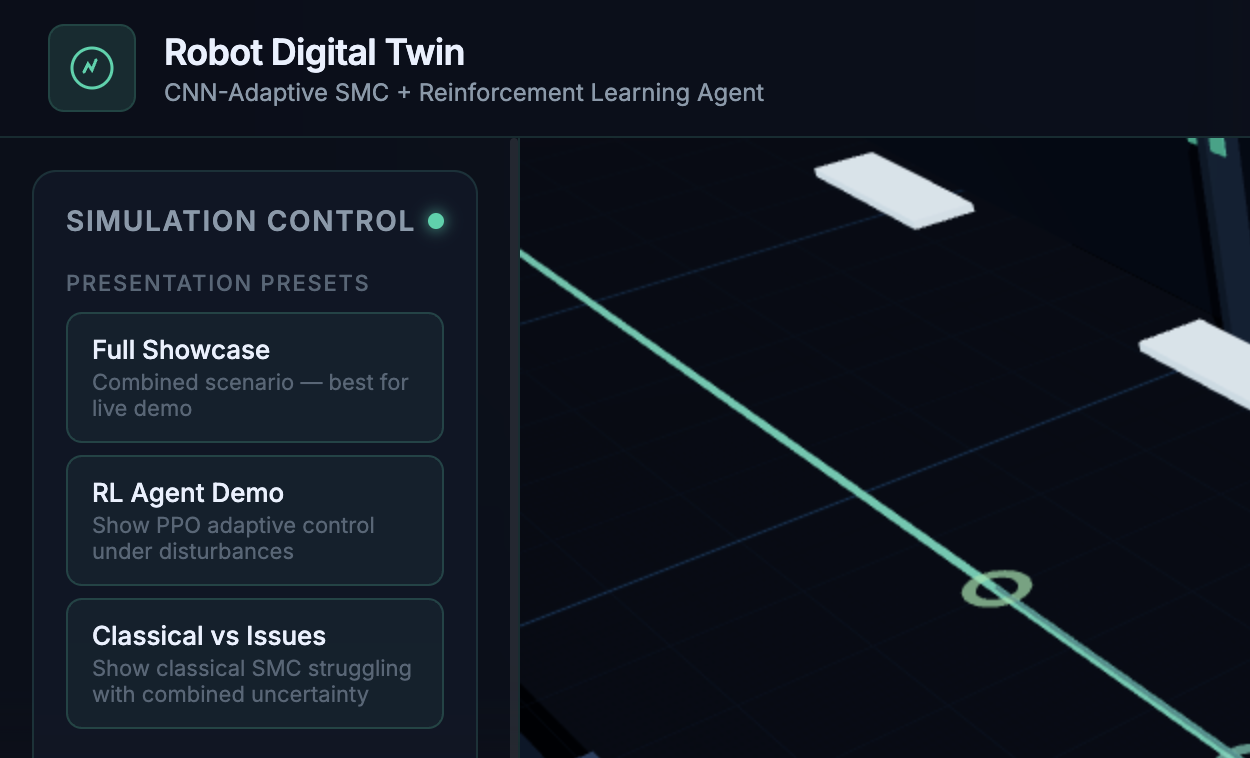
\includegraphics[width=0.92\textwidth]{../assets/figures/fig08_digital_twin.png}
  \caption{3D digital twin interface for live robot simulation, metrics dashboard, and controller comparison.}
  \label{fig:digitaltwin}
\end{figure}

\subsection{Literature Review}

\paragraph{Sliding Mode Control for Mobile Robots.}
SMC provides finite-time convergence and robustness to matched uncertainties~\cite{utkin1992}. Anti-chattering techniques---boundary layers, saturation switching, and higher-order SMC---are well established~\cite{shtessel2014,slotine1991}. Adaptive SMC with Lyapunov-based gain tuning can converge slowly or require tight disturbance bounds~\cite{edwards1998}. Differential-drive platforms benefit from SMC due to nonholonomic constraints and sensitivity to lateral disturbances.

\paragraph{Learning-Based Gain Adaptation.}
Fuzzy-SMC hybrids~\cite{lin2006} and neural-network augmented controllers~\cite{ge2004} tune switching gains automatically. Reinforcement learning combined with SMC has been explored for aerial and manipulation platforms; PPO~\cite{schulman2017} offers stable policy gradient updates for continuous control. A limitation of pure learning approaches is opacity: resulting gain schedules are difficult to interpret or certify, motivating our use of hand-tuned presets selected by a learned classifier.

\paragraph{CNN-Based Supervisory Control.}
Supervisory switching architectures that select among pre-designed controllers based on a mode estimate are established in hybrid systems theory~\cite{liberzon2003}. CNN-based perception has transformed autonomous navigation~\cite{lecun2015,levine2016}, yet direct use of CNN classification for SMC gain scheduling on differential-drive platforms has received comparatively little attention in reproducible student-scale pipelines.

\paragraph{Digital Twins.}
Digital twin technology provides a virtual replica of a physical system for monitoring, simulation, and decision support. For robotics research, a web-based 3D twin enables live demonstration of control algorithms, side-by-side controller comparison, and stakeholder communication during project defense.

\paragraph{Research Gap.}
While SMC, CNN-based perception, and RL-based control have each been studied independently, few projects integrate all three within a unified simulation and visualization platform. This work fills that gap by implementing classical SMC, CNN-adaptive SMC, and PPO-adaptive SMC on the same robot model and evaluating them under identical scenarios.

% ═══════════════════════════════════════
% 2. METHODOLOGY
% ═══════════════════════════════════════
\section{Methodology}

\subsection{Robot and Simulation Model}

The robot is modelled as a unicycle differential-drive with state $\mathbf{q} = [x, y, \theta, v, \omega]^\top$. Continuous-time kinematics:
\begin{equation}
  \dot{x} = v\cos\theta, \quad \dot{y} = v\sin\theta, \quad \dot{\theta} = \omega.
  \label{eq:kinematics}
\end{equation}
Discrete integration uses $\Delta t = 0.01$\,s. Physical parameters: wheel base $L = 0.3$\,m, wheel radius $r = 0.05$\,m. Uncertainty is injected through three mechanisms:
\begin{itemize}
  \item \textbf{Noise:} zero-mean Gaussian noise on pose measurements ($\sigma_{xy}=0.02$\,m, $\sigma_\theta=0.01$\,rad);
  \item \textbf{Disturbance:} single external push of $+0.4$\,m in $y$ at $t=8$\,s;
  \item \textbf{Slip:} 30\% velocity reduction during $t \in [10, 14]$\,s.
\end{itemize}
Five scenarios are evaluated: Normal, Noise, Disturbance, Slip, and Combined (all effects present).

\subsection{CNN-Adaptive SMC Architecture}

Tracking errors are $e_x = x_r - x$, $e_y = y_r - y$, $e_\theta = \theta_r - \theta$. Sliding surfaces:
\begin{equation}
  s_i = \dot{e}_i + \lambda_i e_i, \quad i \in \{x, y, \theta\}.
\end{equation}
The angular velocity command uses hyperbolic-tangent switching to suppress chattering, with exponential smoothing coefficient $\alpha_\omega$.

\begin{figure}[H]
  \centering
  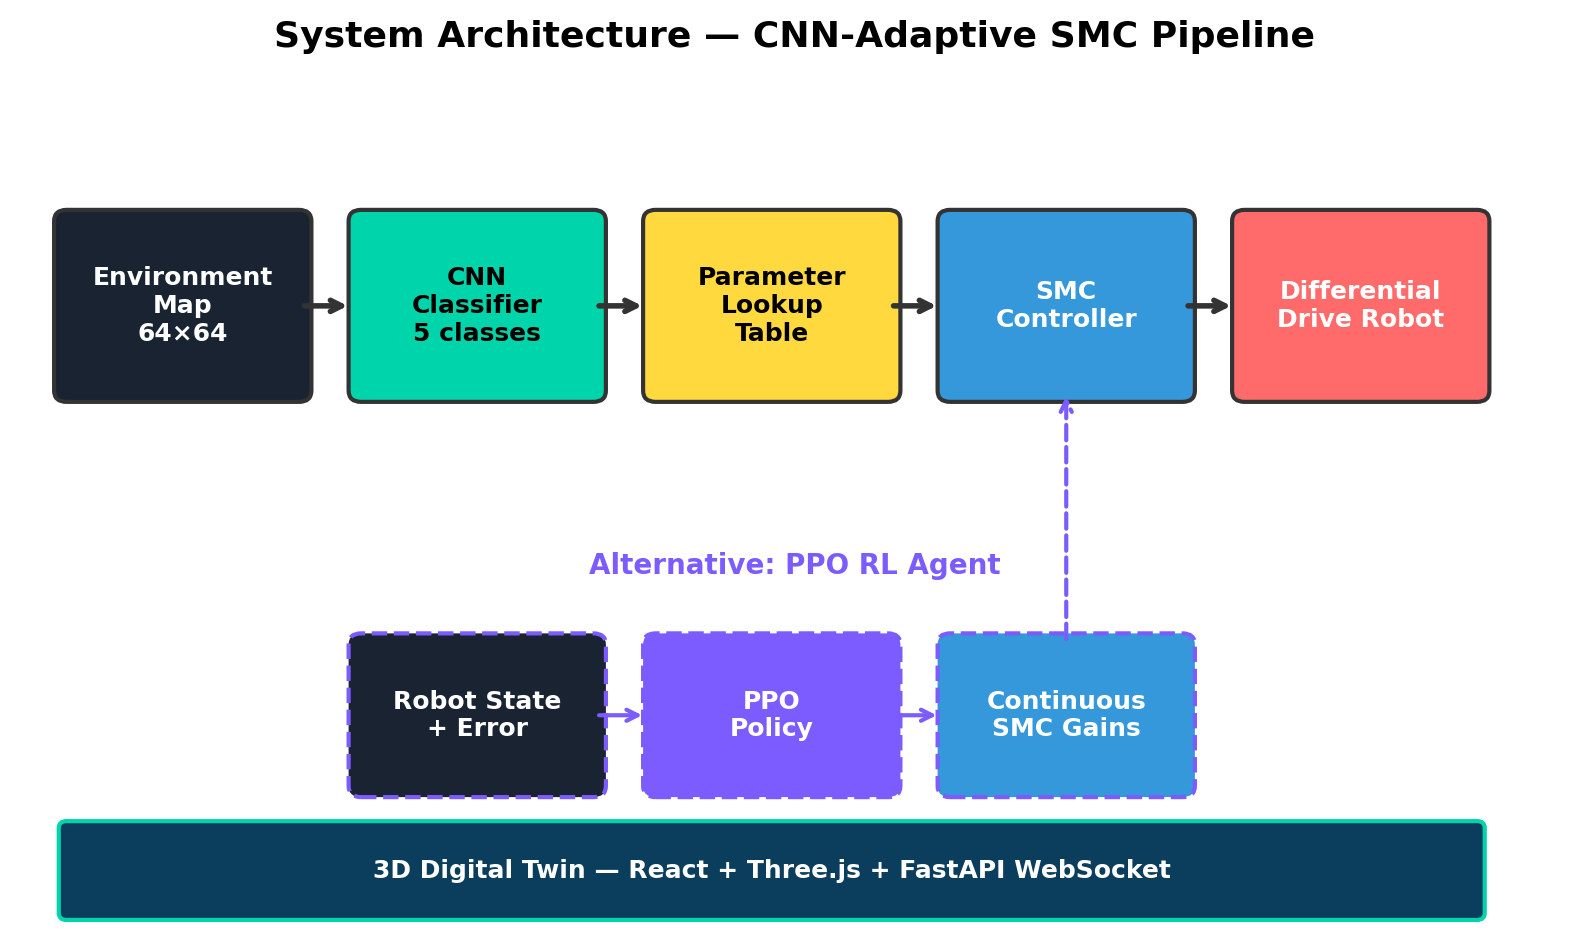
\includegraphics[width=0.95\textwidth]{../assets/figures/fig01_architecture.png}
  \caption{System architecture: CNN classifies a pre-mission map and selects SMC presets; PPO RL provides a continuous alternative; both feed a 3D digital twin.}
  \label{fig:architecture}
\end{figure}

\paragraph{EnvironmentCNN.}
Synthetic 64$\times$64 grayscale maps are generated for five classes (Fig.~\ref{fig:cnnmaps}). The CNN comprises three convolutional blocks (16$\rightarrow$32$\rightarrow$64 filters) with batch normalization, ReLU, max pooling, and a two-layer classifier with dropout ($\approx$534k parameters). Training uses Adam ($\text{lr}=10^{-3}$, batch size 32) with cross-entropy loss.

\begin{figure}[H]
  \centering
  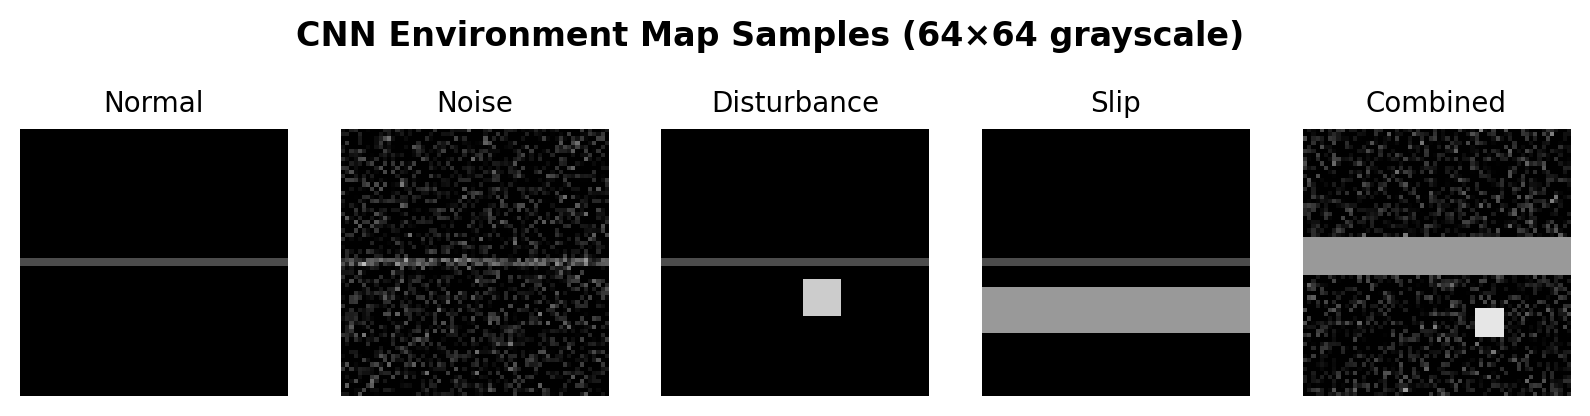
\includegraphics[width=0.95\textwidth]{../assets/figures/fig02_cnn_samples.png}
  \caption{Synthetic environment map samples (one per scenario class) used for CNN training.}
  \label{fig:cnnmaps}
\end{figure}

At deployment, the CNN classifies a pre-mission map and maps the predicted label to a hand-tuned parameter set $\boldsymbol{\pi}_{\hat{c}} = \{\lambda_x, \lambda_y, \lambda_\theta, k_v, k_\omega, \phi, \alpha_\omega\}$. An exponential filter prevents abrupt gain jumps:
\begin{equation}
  \boldsymbol{\pi}_k = (1-\beta)\,\boldsymbol{\pi}_{k-1} + \beta\,\boldsymbol{\pi}_{\hat{c}}, \quad \beta \in (0,1].
\end{equation}

\subsection{Reinforcement Learning Agent (PPO)}

A Gymnasium environment wraps the SMC simulation with domain randomization. The PPO agent uses an actor-critic architecture with Generalized Advantage Estimation (GAE). The per-step reward balances tracking accuracy, control effort, and chattering:
\begin{equation}
  r = -\alpha\, e^2 - \beta\,(v^2 + \omega^2) - \gamma\,|\Delta\omega|.
\end{equation}
Training was performed for 20 iterations with 1024 rollout steps per iteration; the best policy checkpoint was saved to \texttt{models/rl\_smc\_agent.pt}.

\subsection{Digital Twin Platform}

The web-based digital twin (React + Three.js frontend, FastAPI WebSocket backend) provides:
\begin{itemize}
  \item live 3D robot visualization in a hospital corridor environment;
  \item controller tour (Classical $\rightarrow$ CNN $\rightarrow$ RL);
  \item headless benchmark and dual comparison (Classical vs.\ CNN);
  \item simulation replay and CSV export of metrics.
\end{itemize}

\subsection{Evaluation Protocol}

Controllers are compared using: RMSE tracking error, final tracking error, control effort ($\sum|\omega_c|$), and chattering index (variance of successive $\omega_c$ differences). Both controllers track a straight-line reference at $v_r = 0.3$\,m/s for $T = 20$\,s.

% ═══════════════════════════════════════
% 3. RESULTS
% ═══════════════════════════════════════
\section{Results}

\subsection{CNN Classification Performance}

EnvironmentCNN achieved \textbf{100\% validation accuracy} on the synthetic 64$\times$64 map dataset (600 samples, 120 per class) after 12 training epochs. On a more realistic occupancy-grid dataset with obstacles and clutter, the same architecture reaches \textbf{95.1\% test accuracy}, supporting deployability beyond the synthetic benchmark.

\subsection{Classical vs.\ CNN-Adaptive SMC}

Table~\ref{tab:improvement} summarises percentage improvements of CNN-adaptive SMC over classical SMC. Key findings:

\begin{itemize}
  \item \textbf{Noise:} chattering reduced by 35.7\% (76.5 $\rightarrow$ 49.1), with expected RMSE widening due to the smoothness--accuracy trade-off.
  \item \textbf{Disturbance:} final tracking error improved by 14.4\% (20.9\,mm $\rightarrow$ 17.9\,mm), approaching oracle performance (15.6\,mm).
  \item \textbf{Slip:} final error improved by 32.7\% (40.7\,mm $\rightarrow$ 27.4\,mm).
  \item \textbf{Combined:} chattering reduced by 27.1\% with marginal final-error improvement.
\end{itemize}

\begin{table}[H]
  \centering
  \caption{CNN-adaptive improvement over classical SMC (\%). Positive = adaptive better for error metrics; negative chattering = reduction.}
  \label{tab:improvement}
  \small
  \begin{tabular}{@{}lrrrr@{}}
    \toprule
    Scenario & RMSE $\Delta$ & Final Err.\ $\Delta$ & Effort $\Delta$ & Chattering $\Delta$ \\
    \midrule
    Normal       &  0.00 &  0.00 &  0.00 &  0.00 \\
    Noise        & $-$11.7 & $-$130.6$^\dagger$ & $+$5.8 & $+$35.7 \\
    Disturbance  & $+$5.1 & $+$14.4 & $-$5.6 & $-$13.3 \\
    Slip         & $+$2.9 & $+$32.7 & $-$10.9 & $-$23.4 \\
    Combined     & $-$0.9 & $+$1.2 & $-$4.7 & $+$27.1 \\
    \bottomrule
  \end{tabular}\\[0.3em]
  {\footnotesize $^\dagger$Under noise, final error increases in absolute terms (43.7\,mm $\rightarrow$ 100.8\,mm) as an intentional smoothness--accuracy trade-off.}
\end{table}

\begin{figure}[H]
  \centering
  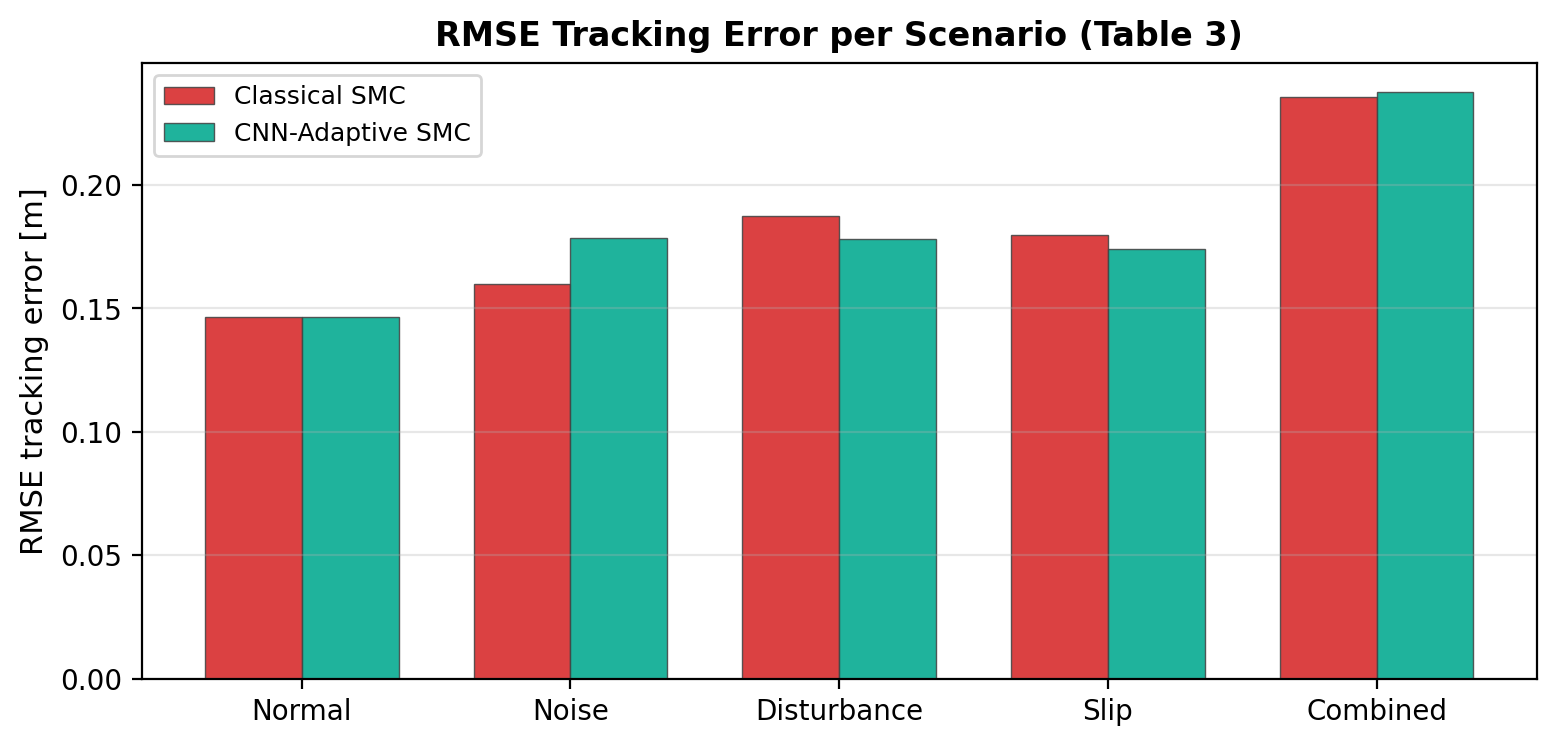
\includegraphics[width=0.48\textwidth]{../assets/figures/fig05_rmse_bars.png}
  \hfill
  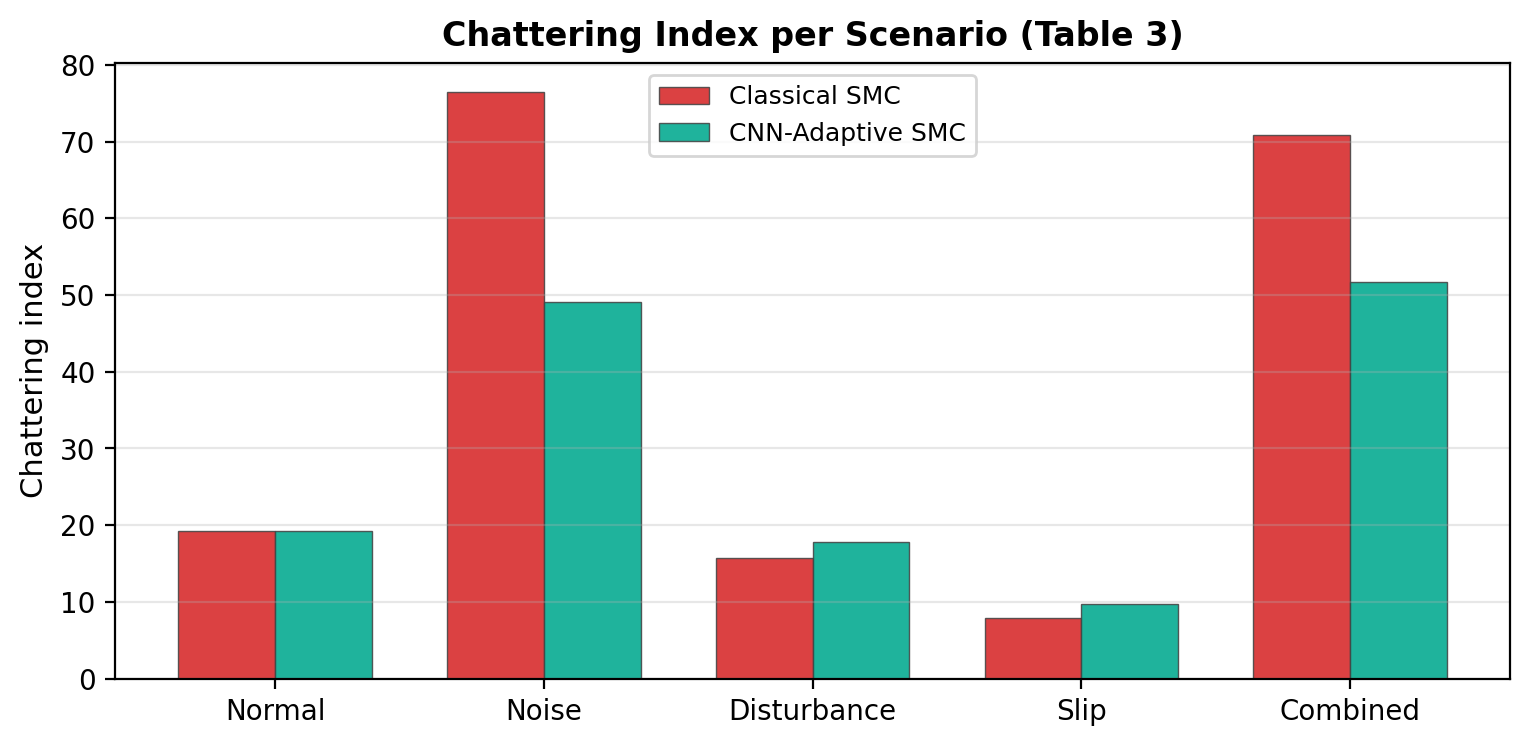
\includegraphics[width=0.48\textwidth]{../assets/figures/fig06_chattering_bars.png}\\[0.4em]
  \caption{Quantitative comparison of classical SMC vs.\ CNN-adaptive SMC: (left) RMSE tracking error; (right) chattering index across five operating scenarios.}
  \label{fig:bars}
\end{figure}

\begin{figure}[H]
  \centering
  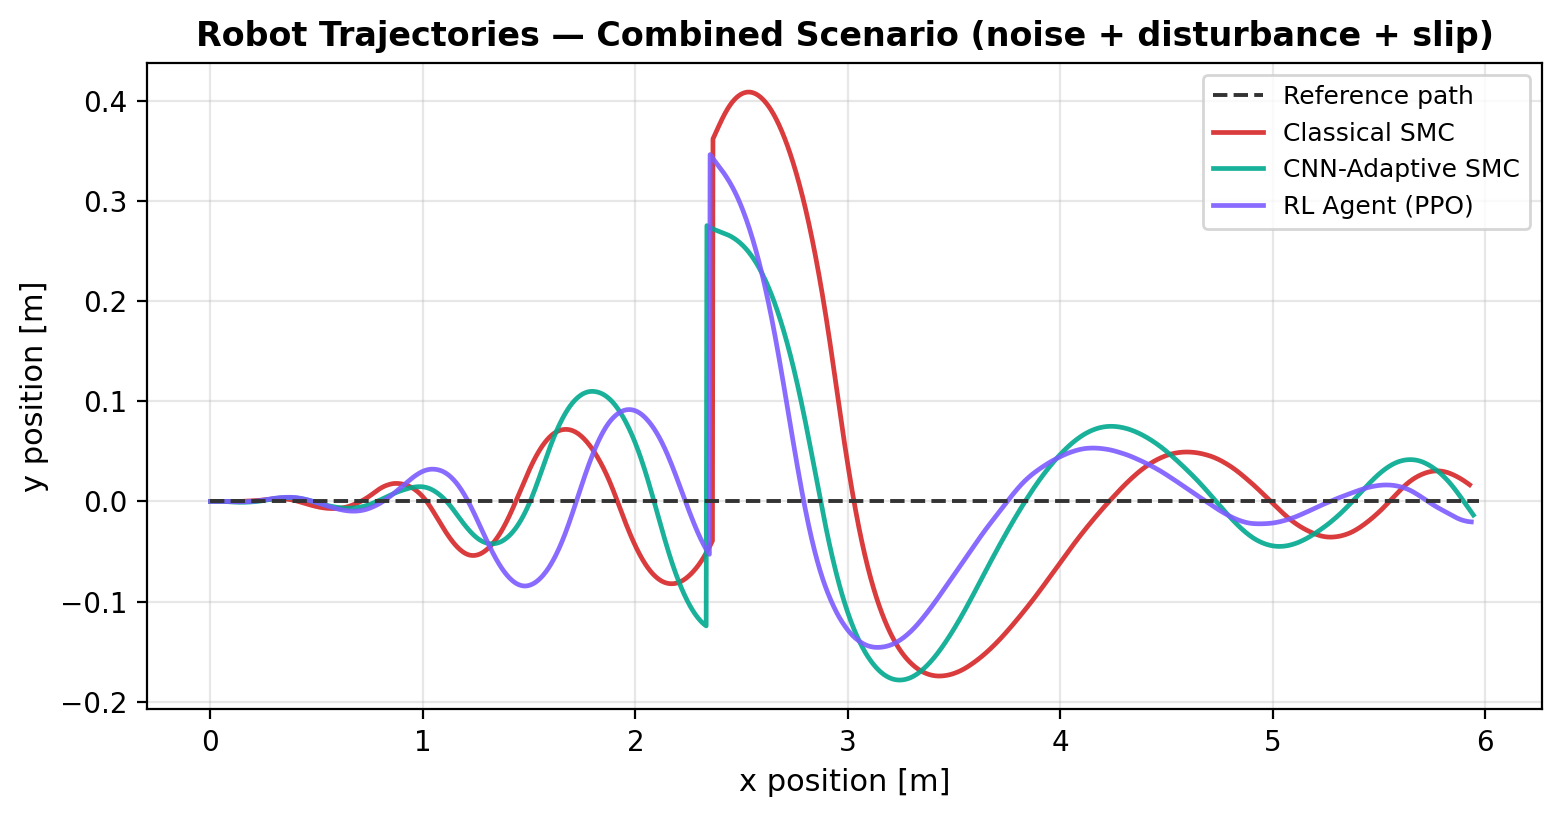
\includegraphics[width=0.88\textwidth]{../assets/figures/fig03_trajectory_comparison.png}
  \caption{Robot trajectories under combined uncertainty for classical SMC, CNN-adaptive SMC, and PPO RL agent.}
  \label{fig:trajectory}
\end{figure}

\begin{figure}[H]
  \centering
  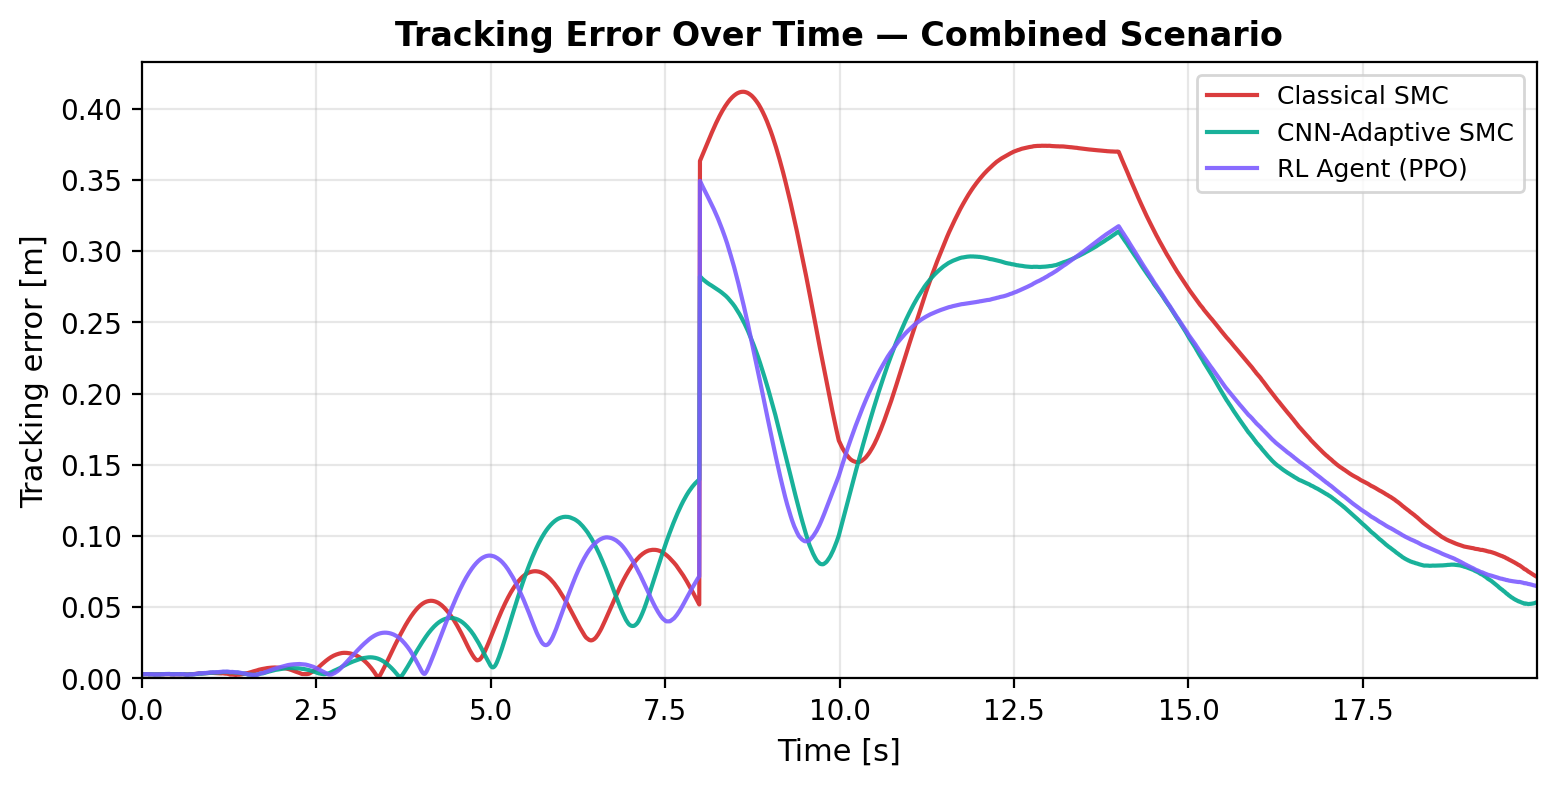
\includegraphics[width=0.88\textwidth]{../assets/figures/fig04_tracking_error.png}
  \caption{Tracking error over time under combined uncertainty. CNN-adaptive SMC shows smoother error profile.}
  \label{fig:error}
\end{figure}

\subsection{Three-Controller Benchmark}

Under the combined scenario (noise + disturbance + slip), classical SMC achieved the lowest RMSE (0.245\,m), while CNN-adaptive SMC achieved the lowest chattering index (30.6). The PPO agent achieved a best mean training reward of $-0.766$ after 20 iterations; longer training and reward shaping are expected to improve RL performance.

\begin{figure}[H]
  \centering
  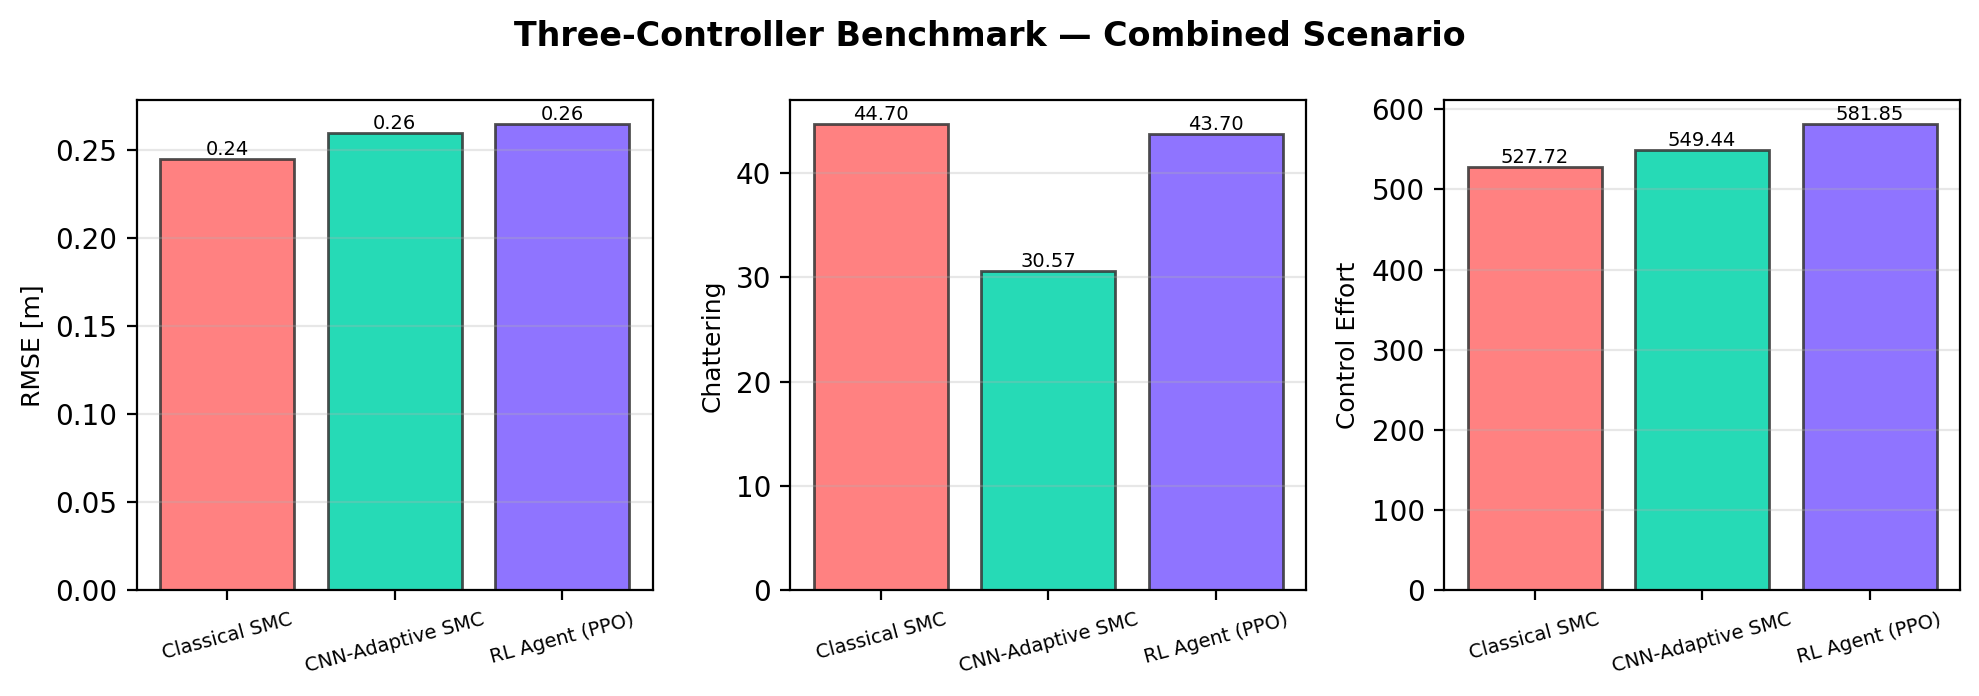
\includegraphics[width=0.88\textwidth]{../assets/figures/fig07_controller_benchmark.png}
  \caption{Headless benchmark of Classical SMC, CNN-Adaptive SMC, and PPO RL agent under combined uncertainty.}
  \label{fig:benchmark}
\end{figure}

\subsection{Multi-Controller Comparison}

Table~\ref{tab:multictrl} compares CNN-adaptive SMC against fuzzy gain scheduling, oracle scenario selection (perfect classification), and RL-based preset selection under identical conditions. Oracle selection establishes the performance ceiling; CNN-adaptive approaches oracle under disturbance and slip recovery.

\begin{table}[H]
  \centering
  \caption{Multi-controller comparison (selected metrics).}
  \label{tab:multictrl}
  \small
  \begin{tabular}{@{}llrrrrr@{}}
    \toprule
    Scenario & Metric & Class. & Fuzzy & CNN & Oracle & RL \\
    \midrule
    Noise        & Chattering index & 76.5 & 70.5 & 49.1 & 49.3 & 50.7 \\
    Disturbance  & Final err.\ (mm) & 20.9 & 24.8 & 17.9 & 15.6 & 32.8 \\
    Slip         & Final err.\ (mm) & 40.7 & 30.4 & 27.4 & 27.4 & 41.6 \\
    Combined     & Chattering index & 72.8 & 71.7 & 51.7 & 51.4 & 48.9 \\
    \bottomrule
  \end{tabular}
\end{table}

% ═══════════════════════════════════════
% 4. CONCLUSIONS
% ═══════════════════════════════════════
\section{Conclusions}

This project designed, implemented, and evaluated a complete intelligent control pipeline for autonomous differential-drive robot navigation:

\begin{itemize}
  \item \textbf{Classical SMC} provides a robust baseline with fixed gains.
  \item \textbf{CNN-adaptive SMC} adds scenario-aware parameter switching, reducing chattering by up to 35.7\% under sensor noise and improving final-error recovery by up to 32.7\% under wheel slip.
  \item \textbf{PPO RL agent} provides a framework for continuous gain adaptation, successfully integrated into the same simulation engine.
  \item \textbf{3D digital twin} enables live demonstration, replay, dual comparison, and CSV export for project defense.
\end{itemize}

The main contribution is an end-to-end research platform---from synthetic dataset generation and CNN training, through multi-controller simulation and quantitative benchmarking, to an interactive 3D digital twin. Results confirm that adaptive control is not uniformly superior on every metric; instead, adaptation enables context-dependent trade-offs valuable in real deployments.

\subsection{Future Work}

\begin{enumerate}
  \item Replace synthetic maps with real LiDAR-based occupancy grids.
  \item Deploy continuous on-line scenario inference for mid-mission condition changes.
  \item Extend RL training with larger scenario randomisation and multi-objective rewards.
  \item Evaluate on curved trajectories with Monte-Carlo repetitions for confidence intervals.
  \item Validate on a physical differential-drive robot.
\end{enumerate}

\vspace{1em}
\noindent\textbf{Project resources.}
\begin{itemize}
  \item \textbf{Digital twin (live demo):} \url{https://smc-cnn.onrender.com}
  \item \textbf{Source code:} \url{https://github.com/LikhitaYerra/smc_cnn}
\end{itemize}

\bibliographystyle{IEEEtran}
\bibliography{references}

\end{document}
